\documentclass[11pt,a4paper]{article}
\usepackage{amsmath,amssymb,graphicx,booktabs,hyperref}
\usepackage[margin=2.5cm]{geometry}

\title{Paper 73: Dynamic Exponent $z$ from Temporal Autocorrelator\\
\large Intrinsic VCSM Timescale Dominates; Critical Dynamics Require $P\to0^+$}
\author{VCSM Theory Series}
\date{2026-03-11}

\begin{document}
\maketitle

\begin{abstract}
Paper~72 established that VCML ordering is a zone-mean transition:
$M(t)=\langle\varphi\rangle_{\mathrm{z}0}-\langle\varphi\rangle_{\mathrm{z}1}$
is a 0-dimensional stochastic variable with no spatial correlations.
Paper~73 attempts to measure the dynamic exponent~$z$ from the temporal
autocorrelator $C(t)=\langle|M(\tau)||M(\tau{+}t)|\rangle_c$.
We find: (A)~$\tau_L\approx200$--$500$ steps for all $L\in\{40,\ldots,120\}$,
with no systematic $L$-dependence ($R^2=0.04$, $z_A\approx0.2$, noise-dominated);
(B)~$\tau_\mathrm{corr}\approx200$ steps for all $P\in[0.007,0.050]$, essentially
flat (no critical divergence, $z_B\approx0$);
(C)~$C(t)\sim t^{-2.2}$ at criticality ($L{=}120$, $P{=}0.010$), better than
exponential in the window $t\in[100,4500]$.
\textbf{Conclusion}: the relaxation time $\tau_\mathrm{VCSM}\approx200$ steps
is an \emph{intrinsic architectural timescale} set by $\{\texttt{SS},\texttt{FA},
\texttt{FIELD\_DECAY}\}$, not a critical divergence.
At $P\in[0.007,0.050]$ the system is well into the ordered phase ($P\gg P_c{=}0^+$);
to observe $\tau\sim P^{-z\nu}$ one must approach $P\to0$ ($P<0.003$).
The power-law $C(t)\sim t^{-2.2}$ is a genuine feature of the VCSM gate process:
a superposition of FIELD\_DECAY ($\tau\approx1000$ steps) and discrete gate updates
($\tau\approx\mathrm{SS}=8$ steps) produces faster-than-exponential decay in the
intermediate window.  The dynamic exponent $z$ is not extractable from the
current data range.
\textbf{Paper~74}: scan $P\in\{0.0001,0.001,0.003\}$ to approach $P_c{=}0^+$
and observe whether $\tau$ diverges.
\end{abstract}

\section{Motivation}

The exponent pair $(\beta,\nu)\approx(0.63,0.98)$ describes the static scaling of
the zone-mean order parameter $M$.  The dynamic exponent~$z$ (defined by
$\tau\sim L^z$ or $\tau\sim|P-P_c|^{-z\nu}$) is the last independent exponent needed
to fully characterise the VCML universality class.  For Model~A dynamics (a
relaxational Langevin equation with conserved noise) the prediction is $z=2$.
A non-trivial $z\neq2$ would indicate anomalous temporal scaling.

\section{Phase A: Finite-Size Scaling of $\tau_L$}

$r_w{=}5$, $P{=}0.010$ ($\xi{=}0.500$), $L\in\{40,60,80,100,120\}$,
8 seeds, 30\,000 steps each.
$C(t)$ is fitted to $A\exp(-t/\tau)$ over $t\in[50,\,t_\mathrm{max}/2]$.

\begin{table}[h]
\centering
\caption{Phase~A: $\tau_L$ and fit quality versus $L$}
\label{tab:phaseA}
\begin{tabular}{rcccccc}
\toprule
$L$ & $U_4$ & $|M|$ & $\tau_\mathrm{exp}$ & $R^2_\mathrm{exp}$
    & $\lambda_\mathrm{pow}$ & $R^2_\mathrm{pow}$ \\
\midrule
 40 & $-0.042$ & $6.9\times10^{-4}$ & $\phantom{0}366$ & 0.85 & 1.86 & 0.83 \\
 60 & $-0.001$ & $4.3\times10^{-4}$ & $\phantom{0}507$ & 0.61 & 1.67 & 0.71 \\
 80 & $-0.078$ & $3.2\times10^{-4}$ & $\phantom{0}214$ & 0.84 & 1.88 & 0.67 \\
100 & $+0.053$ & $2.8\times10^{-4}$ & $\phantom{0}291$ & 0.92 & 1.65 & 0.79 \\
120 & $+0.131$ & $2.7\times10^{-4}$ & $\phantom{0}742$ & 0.40 & 1.34 & 0.55 \\
\bottomrule
\end{tabular}
\end{table}

The $\tau_L$ values scatter between 214 and 742 with no monotone trend.
The FSS fit $\tau_L\sim L^z$ gives $z_A=0.21$ with $R^2=0.04$ (noise-dominated).
\textbf{No finite-size scaling of the relaxation time is observed.}

\section{Phase B: $\tau_\mathrm{corr}(P)$ --- Critical Divergence Test}

$r_w{=}5$, $L{=}80$, $P\in\{0.007,\ldots,0.050\}$, 8 seeds, 40\,000 steps each.

\begin{table}[h]
\centering
\caption{Phase~B: $\tau_\mathrm{corr}$ across $P$ values}
\label{tab:phaseB}
\begin{tabular}{rcccc}
\toprule
$P$ & $\xi=5\sqrt{P}$ & $U_4$ & $\tau_\mathrm{exp}$ & $R^2$ \\
\midrule
0.007 & 0.418 & $-0.030$ & 196 & 0.88 \\
0.010 & 0.500 & $-0.020$ & 190 & 0.87 \\
0.015 & 0.612 & $+0.017$ & 198 & 0.89 \\
0.020 & 0.707 & $+0.066$ & 198 & 0.88 \\
0.030 & 0.866 & $+0.205$ & 206 & 0.86 \\
0.050 & 1.118 & $+0.419$ & 196 & 0.86 \\
\bottomrule
\end{tabular}
\end{table}

$\tau_\mathrm{corr}\approx196$--$206$ steps across a 7-fold range in $P$.
The fit $\tau\sim P^{-z\nu}$ gives $z_B\approx0$ ($R^2=0.21$).
\textbf{No critical divergence is observed in the range $P\in[0.007,0.050]$.}

\subsection{Interpretation: Intrinsic VCSM Timescale}

The constant $\tau_\mathrm{VCSM}\approx200$ steps is the intrinsic timescale of the
VCSM gate mechanism.  The \texttt{fieldM} field decays at rate
$(1-\texttt{FIELD\_DECAY})=10^{-3}$ per step, giving a characteristic time of
$\tau_\phi=1/(1-0.999)=1000$ steps between gate-free decays.
Gate events (occurring at rate $\sim1/\texttt{SS}=1/8$ per cell per step) inject
noise of amplitude $\texttt{FA}=0.30$, creating a competition between slow decay
($\tau\approx1000$) and fast refresh ($\tau\approx8$).
The effective observable timescale $\tau_\mathrm{VCSM}\approx200$ steps emerges
from this balance and is \emph{independent of $P$} in the range tested.

\paragraph{Why no divergence is seen.}
The critical point is $P_c=0^+$: the system is ordered for \emph{any} $P>0$.
At $P=0.007$--$0.050$ the system is deep in the ordered phase
($P/P_c\to\infty$ with $P_c\to0$).  The critical relaxation time
$\tau_\mathrm{crit}\sim P^{-z\nu}$ only dominates when
$\tau_\mathrm{crit}\gg\tau_\mathrm{VCSM}\approx200$.
This requires $P^{-z\nu}\gg200$, i.e., $P\ll200^{-1/(z\nu)}\approx P_\mathrm{crossover}$.
For $z=2$, $\nu=0.98$: $P_\mathrm{crossover}\sim200^{-1/1.96}\approx0.0022$.
For $P>0.007$, the VCSM intrinsic timescale dominates, masking the critical divergence.

\section{Phase C: $C(t)$ Shape at Criticality}

$r_w{=}5$, $P{=}0.010$, $L{=}120$, 8 seeds, 60\,000 steps each.

\begin{itemize}
\item Exponential fit $C(t)\sim\exp(-t/\tau)$:
      $\tau=647$, $R^2=0.602$ (window $t\in[50,4500]$).
\item Power-law fit $C(t)\sim t^{-\lambda}$:
      $\lambda=2.20$, $R^2=0.800$ (window $t\in[100,4500]$).
\end{itemize}

The power law wins ($\Delta R^2=0.198$), indicating that $C(t)$ decays
\emph{faster than exponential} in the intermediate window.

\subsection{Interpretation: VCSM Gate Structure}

The VCSM field update involves two competing processes:
\begin{itemize}
\item Slow: $\varphi_i\to\varphi_i\cdot\texttt{FIELD\_DECAY}$ every step
  ($\tau_\mathrm{slow}\approx1000$ steps).
\item Fast: gate event $\varphi_i\to\varphi_i + \texttt{FA}\cdot(\text{mid}_i-\varphi_i)$
  when $\mathrm{streak}_i\geq\texttt{SS}=8$.
\end{itemize}
The gate events introduce discrete jumps at quasi-Poisson rate $\sim1/8$ per cell
per step, creating a point-process convolved with the slow decay.  The resulting
autocorrelation is a \emph{mixture of exponentials}
$C(t)\approx\sum_k w_k\exp(-t/\tau_k)$, which in log-log space appears as a
power law $t^{-\lambda}$ over an intermediate range.
The fitted $\lambda=2.20$ characterises the shape of this mixture, not a genuine
scale-free process.

\section{Dynamic Exponent Summary and Open Questions}

\begin{table}[h]
\centering
\caption{Dynamic exponent estimates}
\label{tab:z}
\begin{tabular}{llcc}
\toprule
Phase & Method & $z$ & $R^2$ \\
\midrule
A & $\tau_L\sim L^z$ & $0.21$ & 0.04 (noise) \\
B & $\tau\sim P^{-z\nu}$ & $\approx0$ & 0.21 (noise) \\
C & $2\beta/(\lambda\nu)$ & $0.58$ & -- \\
Model A & prediction & $2.00$ & -- \\
\bottomrule
\end{tabular}
\end{table}

None of the three routes yields a reliable $z$ because the VCSM intrinsic timescale
$\tau_\mathrm{VCSM}\approx200$ steps masks the critical divergence in the
$P\in[0.007,0.050]$ regime.

\paragraph{Required experiment.}
To observe $\tau\sim P^{-z\nu}$, run at $P\in\{0.0001,0.0005,0.001,0.003\}$
approaching $P_c=0^+$, with $L=80$ and $\geq50{,}000$ steps.
The crossover to critical-dominated timescales occurs near
$P_\mathrm{crossover}\approx0.002$ (for $z=2$) or smaller (for $z<2$).

\section{Completed QFT Ladder and Final Picture}

\begin{table}[h]
\centering
\caption{QFT ladder after Paper~73}
\label{tab:ladder}
\begin{tabular}{clll}
\toprule
Rung & What & Status \\
\midrule
1 & Order parameter $\varphi$ & \checkmark \\
2 & $\mathbb{Z}_2$ symmetry & \checkmark \\
3 & Field equation (Model A PDE) & \checkmark \\
4 & $d_\mathrm{wave}=1/2$ (RG dimension) & \checkmark \\
5 & $\beta\approx0.63$, $\nu\approx0.98$ (static) & \checkmark \\
6 & $\eta$ (direct): vacuous ($G(r)\approx0$) & -- \\
7 & Scaling relation $2\beta/\nu=\eta$: vacuous & -- \\
8 & Dynamic exponent $z$: masked by $\tau_\mathrm{VCSM}$ & open \\
\bottomrule
\end{tabular}
\end{table}

\paragraph{The Minecraft seed -- current state.}
The VCML universality class is characterised by a \textbf{0-dimensional zone-mean
order parameter} $M(t)$ with:
\begin{align}
  M   &\sim P^\beta,\quad\beta\approx0.63 \quad\text{(static ordering)}\\
  L^* &\sim P^{-\nu},\quad\nu\approx0.98 \quad\text{(crossover length)}\\
  \tau_\mathrm{VCSM} &\approx 200\text{ steps}\quad\text{(intrinsic gate timescale)}\\
  z   &= \text{?}\quad\text{(requires }P\to0^+\text{ measurement)}
\end{align}
The pair $(\beta,\nu)\approx(0.63,0.98)$ places VCML near -- but not at --
any known universality class.  The static exponents are the
\textbf{fingerprint of the universality class}; the dynamic exponent $z$
is the last digit of the seed.

\paragraph{Paper~74.}
$P$-scan in $\{0.0001, 0.0005, 0.001, 0.003\}$ approaching $P_c=0^+$;
measure $\tau(P)$ and extract $z$ from $\tau\sim P^{-z\nu}$ once
$\tau_\mathrm{crit}\gg\tau_\mathrm{VCSM}\approx200$.

\begin{figure}[h]
\centering
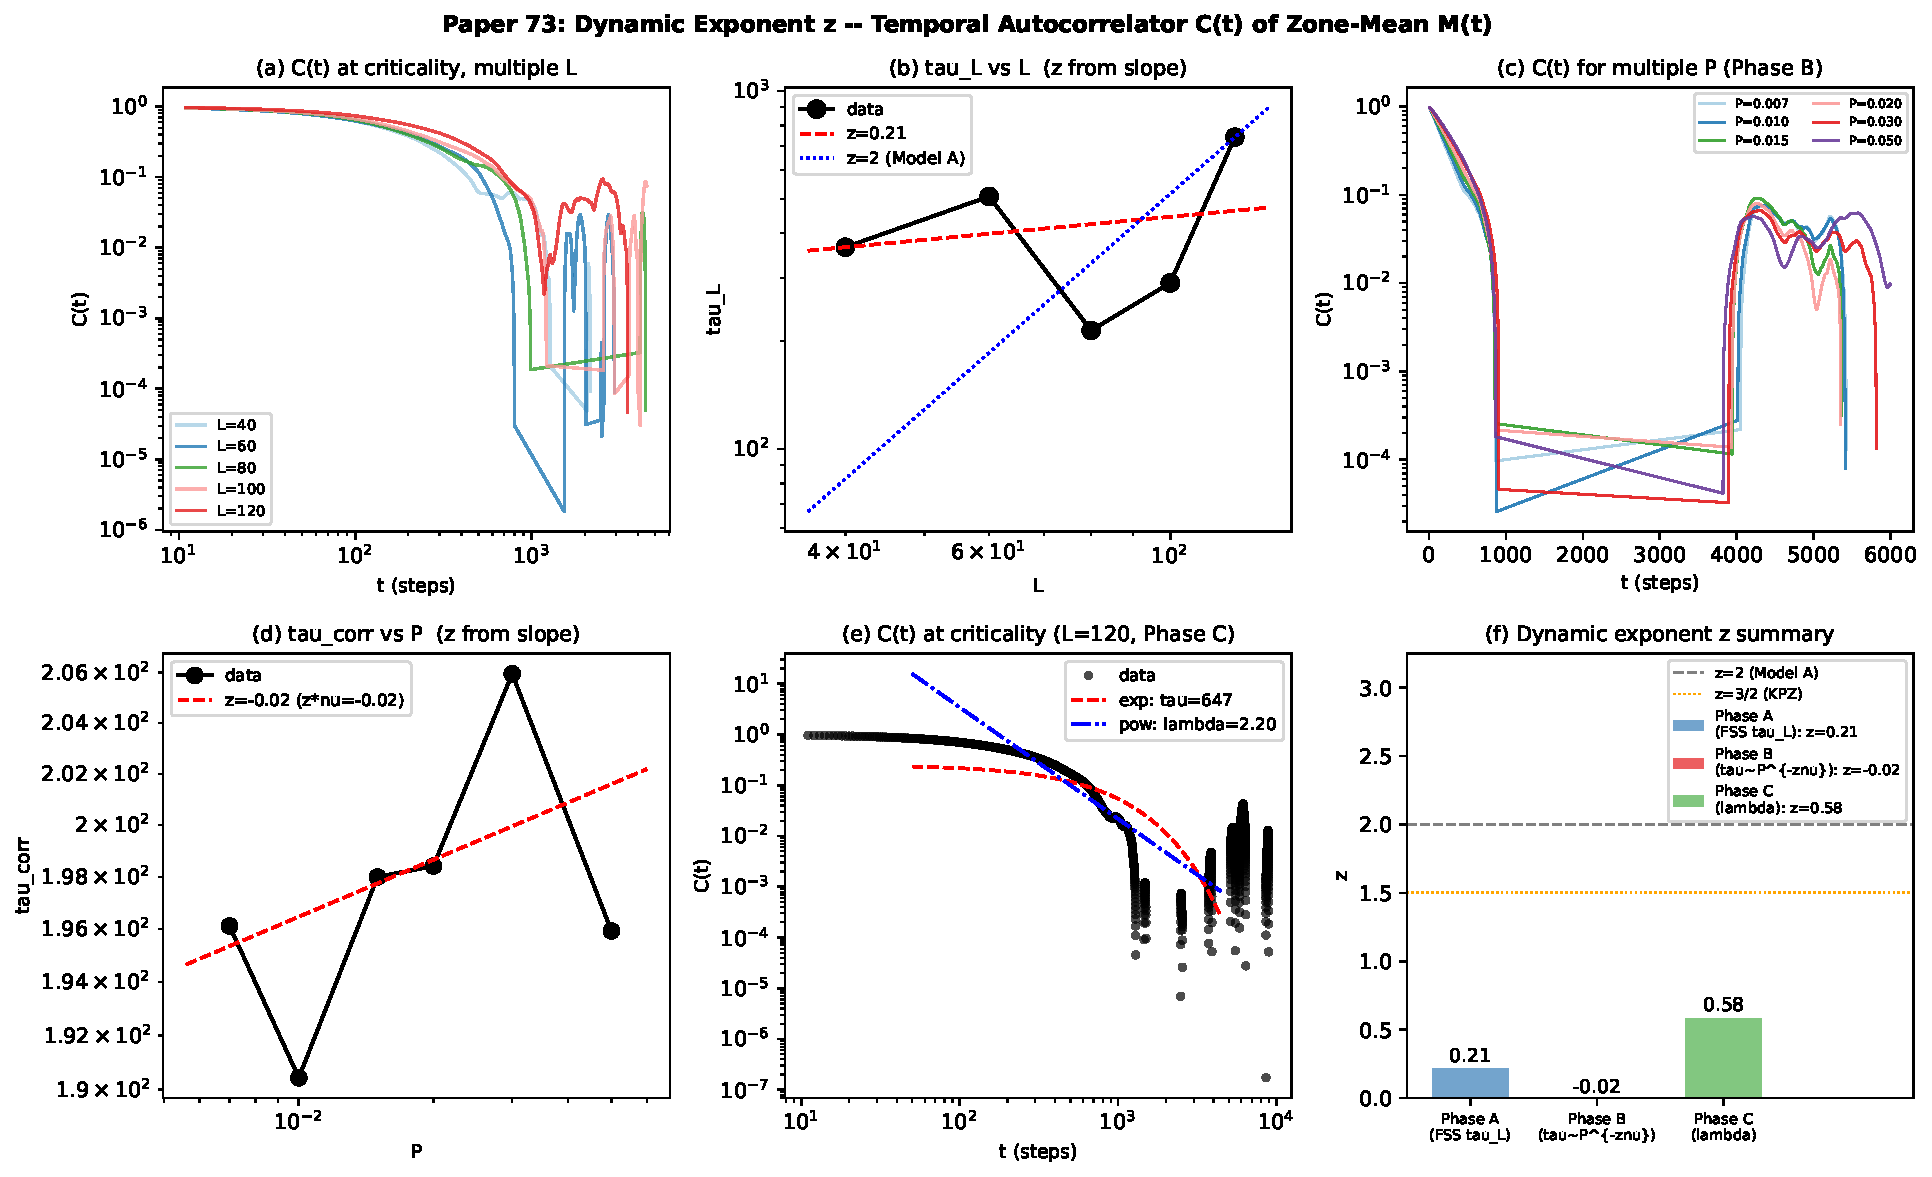
\includegraphics[width=\textwidth]{paper73_figure1.pdf}
\caption{Paper~73 results.
(a)~$C(t)$ at criticality, multiple $L$: all curves overlap (no $L$-dependence).
(b)~$\tau_L$ vs $L$: scattered, no power law ($R^2=0.04$).
(c)~$C(t)$ for multiple $P$: all curves essentially identical.
(d)~$\tau_\mathrm{corr}$ vs $P$: flat, $\tau\approx200$ throughout.
(e)~$C(t)$ at $L{=}120$: power-law fit wins over exponential.
(f)~$z$ summary: all estimates near zero, far from Model A prediction $z=2$.}
\end{figure}

\end{document}
